\everymath{\displaystyle}

%%%%%%%%%%%%%%%%%%%%%%%%%%%%%%%%%%%%%%%%
%           main body
%%%%%%%%%%%%%%%%%%%%%%%%%%%%%%%%%%%%%%%%

%-----------------------------------
%	TITLE PAGE
%-----------------------------------

\title[数学分析研讨课]{\texorpdfstring{\Huge \bfseries 2026年春季学期 -- 数学分析研讨课}{2026年春季学期 -- 数学分析研讨课}} % The short title appears at the bottom of every slide, the full title is only on the title page
\author[解析数论] % Your institution as it will appear on the bottom of every slide, maybe shorthand to save space
{\huge \bfseries 主题: 解析数论 (Analytic Number Theory)}
% \author{Singular Value Decomposition} % Your name
% \date{\today} % Date can be changed to a custom date
\date{}

%------------------------------------------------

\begin{document}

%------------------------------------------------

\begin{frame}

\titlepage % Print the title page as the first slide

\end{frame}

%------------------------------------------------

% \begin{frame}
% \frametitle{内容提要} % Table of contents slide, comment this block out to remove it
% \tableofcontents % Throughout your presentation, if you choose to use \section{} and \subsection{} commands, these will automatically be printed on this slide as an overview of your presentation
% \end{frame}

%-----------------------------------
%	PRESENTATION SLIDES
%-----------------------------------

\section{课程简介与课程大纲}

%------------------------------------------------

\begin{frame}
\frametitle{课程简介}

\begin{itemize}
\item \textbf{主题}: 解析数论引论 (Introduction to Analytic Number Theory)
\item \textbf{教材}: \textit{Introduction to Analytic Number Theory}, A. J. Hildebrand (Lecture Notes)
\item \textbf{预备知识}: 数学分析, 复变函数, 初等数论, 以及一些基本的代数和组合学知识.
\item \textbf{形式}: 报告 (PPT 或者板书) + 讨论
\item \textbf{分组}: 2人一组, 共14周 (Week 2 -- Week 15)
\item \textbf{考核}: 课堂报告表现 + 期末小论文/总结
\pause
\item \textbf{英文参考书}:
\begin{itemize}
\item Apostol, \textit{Introduction to Analytic Number Theory}.
\item Montgomery \& Vaughan, \textit{Multiplicative Number Theory}.
\item Davenport, \textit{Multiplicative Number Theory}.
\end{itemize}
\item \textbf{中文参考书}:
\begin{itemize}
\item 潘承洞, 潘承彪, 《解析数论基础》.
\item 华罗庚, 《数论导引》.
\item 加藤和也 等, 《数论I：Fermat的梦想与类域论》.
\end{itemize}
\end{itemize}

\end{frame}

%------------------------------------------------

\begin{frame}
\frametitle{课程大纲}

\begin{itemize}
\item \textbf{Week 1}: 导论 (Introduction): primes, Euler product, zeta function
\item \textbf{Week 2}: Primes \& Arithmetic Functions Basics (0.1--0.3, 1.1--1.2).
\item \textbf{Week 3}: Möbius Function, Euler $\varphi$ Function (1.3--1.4).
\item \textbf{Week 4}: Dirichlet Convolution, von Mangoldt Function (1.5--1.7).
\item \textbf{Week 5}: Asymptotic Estimates, Big-O, Euler Summation (2.1--2.2).
\item \textbf{Week 6}: Summation by Parts (2.3).
\item \textbf{Week 7}: Convolution Method, Squarefree Integers (2.4).
\item \textbf{Week 8}: Dirichlet Hyperbola Method, Divisor Problem (2.5).
\item \textbf{Week 9}: Chebyshev Estimates for Primes (3.1).
\item \textbf{Week 10}: Mertens Estimates (3.2--3.4).
\item \textbf{Week 11}: Dirichlet Series: Algebraic Properties (4.1--4.2).
\item \textbf{Week 12}: Dirichlet Series: Analytic Properties, Mellin Transform (4.3--4.4).
\item \textbf{Week 13}: Riemann Zeta Function: Basic \& Upper Bounds (5.1--5.3).
\item \textbf{Week 14}: Zero-free Region \& PNT Idea (5.4--5.5).
\item \textbf{Week 15}: (Backup/Review) Dirichlet's Theorem on Primes in AP (Ch. 6 intro).
\end{itemize}

\end{frame}

%------------------------------------------------

\section{课程引论: 解析数论概览}

% Part 1
\begin{frame}
\frametitle{1. 素数计数问题与素数定理}
\begin{itemize}
\item \textbf{问题}: 研究不超过 $x$ 的素数个数 $\pi(x) = \sum_{p \le x} 1$ 的渐近行为.
\item \textbf{数值观察}:
\begin{center}
\begin{tabular}{c|c|c|c}
$x$ & $\pi(x)$ & $x/\log x$ & $\pi(x) / (x/\log x)$ \\
\hline
10 & 4 & 4.34 & 0.921 \\
100 & 25 & 21.7 & 1.151 \\
1000 & 168 & 144.8 & 1.161 \\
$10^6$ & 78,498 & 72,382 & 1.084 \\
\end{tabular}
\end{center}
\item \textbf{素数定理 (Prime Number Theorem, PNT)}:
\begin{alertblock}{PNT}
\[
\pi(x) \sim \frac{x}{\log x} \quad (x \to \infty).
\]
\end{alertblock}
\item \textbf{注记}: 这是一个关于\alert{离散}整数集合分布规律的定理, 但其证明的关键步骤却依赖于\alert{复分析}的工具.
\end{itemize}
\end{frame}


\begin{frame}
\frametitle{1. 素数计数问题与素数定理}

关于素数定理: 是 Gau{\ss} 最早猜测 $\pi(x) \sim \frac{x}{\log x}$, 但如果考虑素数密度随位置变化 (局部概率密度约为 $\frac{1}{\log x}$), 则更自然的猜测是 $\pi(x) \sim \mathrm{Li}(x)$, 其中 $\mathrm{Li}(x) = \int_2^x \frac{dt}{\log t}$ 是素数计数函数的更精确近似. 事实上, $\mathrm{Li}(x)$ 与 $x/\log x$ 的比值趋于1, 但 $\mathrm{Li}(x)$ 的误差项更小.

\begin{center}

\includegraphics[width=0.55\textwidth]{images/pnt_plot.pdf}
\end{center}

\end{frame}

% Part 2
\begin{frame}
\frametitle{2. Euler 乘积公式: 算术基本定理的分析形式}
\begin{itemize}
\item \textbf{几何级数展开}: 对于每个素数 $p$, 我们有:
\[
\left(1 - \frac{1}{p^s}\right)^{-1} = 1 + \frac{1}{p^s} + \frac{1}{p^{2s}} + \frac{1}{p^{3s}} + \cdots
\]
\item \textbf{Euler Product}: 将所有素数的因子相乘 (利用算术基本定理):
\[
\prod_{p} \left(1 - p^{-s}\right)^{-1} = \prod_{p} \left( \sum_{k=0}^\infty p^{-ks} \right) = \sum_{n=1}^\infty \frac{1}{n^s} = \zeta(s).
\]
\item \textbf{意义}: $\zeta(s)$ 将\alert{素数的乘法结构}转化为了\alert{自然数的加法结构}.
\end{itemize}
\end{frame}

% Part 3
\begin{frame}
\frametitle{3. Riemann $\zeta$ 函数与零点}
Riemann (1859) 的两个关键思想:
\begin{enumerate}
\item 将 $\zeta(s)$ \textbf{解析延拓} (Analytic Continuation) 到整个复平面 $\mathbb{C}$.
\item 研究 $\zeta(s)$ 的\textbf{零点}分布.
\end{enumerate}

\begin{alertblock}{Riemann Hypothesis (RH)}
$\zeta(s)$ 的所有非平凡零点 (Non-trivial Zeros) 都位于临界线 $\mathrm{Re}(s) = \frac{1}{2}$ 上.
\end{alertblock}

\begin{itemize}
\item RH 若成立, 意味着素数的分布误差项 $\pi(x) - \mathrm{Li}(x)$ 达到最优估计 $O(x^{1/2+\epsilon})$.
\end{itemize}
\end{frame}

% Part 4
\begin{frame}
\frametitle{4. 解析数论的方法论: Tauber 型定理}
解析数论的核心哲学 (Heuristic):
\[
\text{函数 } F(s) \text{ 的解析性质} \iff \text{系数 } a_n \text{ 的算术性质}
\]

\begin{exampleblock}{一个直观的例子}
\[
-\frac{\zeta'}{\zeta}(s) \text{ 在 } s=1 \text{ 处有简单极点} \implies \pi(x) \sim \frac{x}{\log x}.
\]
\end{exampleblock}

\begin{itemize}
    \item 这种通过生成函数的极点、留数来反推部分和 $A(x) = \sum_{n \le x} a_n$ 渐近行为的定理, 统称为 \textbf{Tauberian Theorems}.
\end{itemize}
\end{frame}

% Part 5
\begin{frame}
\frametitle{5. 分析与代数的联系: 类数公式}
在数学分析\textbf{无穷乘积}一节中曾提到 $\sin x$ 的乘积展开:
\[
\frac{\sin(\pi x)}{\pi x} = \prod_{n=1}^\infty \left( 1 - \frac{x^2}{n^2} \right) \implies \zeta(2) = \frac{\pi^2}{6}.
\]
更进一步, 它与代数数论中的\textbf{类数公式} (Class Number Formula) 密切相关.
\begin{itemize}
    \item 对于虚二次域 $K = \mathbb{Q}(\sqrt{D})$ ($D < 0$ 为判别式), 其 $L$-函数在 $s=1$ 处的值为:
    \[
    L(1, \chi_{D}) = \frac{2\pi h_K}{w \sqrt{|D|}}.
    \]
    \item 这里 $h_K$ 是 $K$ 的\alert{理想类群} (Ideal Class Group) 的阶, 衡量了 $K$ 中唯一分解定理失效的程度.
    \item 例如: Leibniz 级数 $1 - \frac{1}{3} + \frac{1}{5} - \cdots = \frac{\pi}{4}$ 对应 $\mathbb{Q}(i)$ (即 $D=-4$), 此时 $h_K=1, w=4, \sqrt{|D|}=2$.
\end{itemize}
\end{frame}

% Part 7
\begin{frame}
\frametitle{课程脉络}
本课程的研讨路线:
\begin{center}
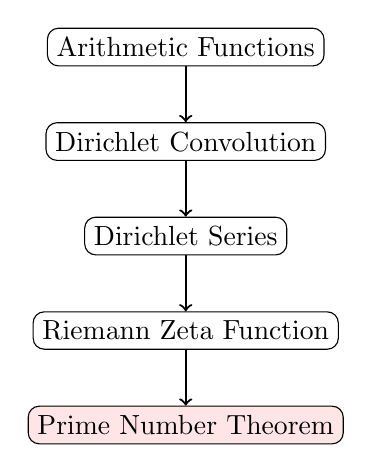
\begin{tikzpicture}[node distance=1.2cm, auto]
\node (arith) [draw, rounded corners] {Arithmetic Functions};
\node (conv) [draw, rounded corners, below of=arith] {Dirichlet Convolution};
\node (series) [draw, rounded corners, below of=conv] {Dirichlet Series};
\node (zeta) [draw, rounded corners, below of=series] {Riemann Zeta Function};
\node (pnt) [draw, rounded corners, fill=red!10, below of=zeta] {Prime Number Theorem};

\draw[->, thick] (arith) -- (conv);
\draw[->, thick] (conv) -- (series);
\draw[->, thick] (series) -- (zeta);
\draw[->, thick] (zeta) -- (pnt);
\end{tikzpicture}
\end{center}
\textbf{核心目标}: 理解 $\zeta(s)$ 的解析性质如何控制素数的分布规律.
\end{frame}

%------------------------------------------------

\section{课程内容详述}

\begin{frame}
\frametitle{第一阶段: 算术函数的代数理论 (Week 1-4)}
\textbf{重点: 建立算术函数的代数结构, 不涉及复杂分析.}
\begin{itemize}
    \item \textbf{Week 2 (基础)}: 积性函数 (Multiplicative Functions). 算术基本定理保证了积性函数由其在素数幂处的值完全决定.
    \item \textbf{Week 3 (Möbius 反演)}: $\mu(n)$ 不仅是一个函数, 它是 Dirichlet 卷积下的``除法''. 解决``已知 $g = f * 1$, 反求 $f$'' 的问题.
    \item \textbf{Week 4 (Dirichlet 卷积)}: 证明所有算术函数在卷积下构成一个环. 这是后续 Dirichlet 级数理论的代数基础.
\end{itemize}
\end{frame}

\begin{frame}
\frametitle{第二阶段: 初等渐近估计方法 (Week 5-8)}
\textbf{重点: 利用实变量微积分估计数论和式.}
\begin{itemize}
    \item \textbf{Week 5 (求和公式)}: Euler Summation Formula. 如何将离散求和 $\sum_{n \le x} f(n)$ 转化为积分 $\int f(t)dt$ 加上误差项.
    \item \textbf{Week 6 (分部求和)}: Summation by Parts (Abel Summation). 处理 $\sum a_n f(n)$ 的最强初等工具, 离散版本的分部积分法.
    \item \textbf{Week 7 (卷积法)}: 处理 $\sum \varphi(n)$ 等平均值问题. 技巧是将复杂函数分解为简单函数的卷积 ($\varphi = \mu * \mathrm{Id}$).
    \item \textbf{Week 8 (双曲线法)}: Dirichlet Hyperbola Method. 专门处理除数函数 $d(n)$ 的求和, 几何上对应于双曲线 $xy \le x$ 下的整点计数.
\end{itemize}
\end{frame}

\begin{frame}
\frametitle{第三阶段: 素数分布的初等结果 (Week 9-10)}
\textbf{重点: 在引入复变函数之前, 我们能对素数知道多少?}
\begin{itemize}
\item \textbf{Week 9 (Chebyshev 估计)}: 虽然无法初等证明 $\pi(x) \sim x/\log x$, 但 Chebyshev 证明了其量级确实是 $x/\log x$, 即 $c_1 \frac{x}{\log x} < \pi(x) < c_2 \frac{x}{\log x}$.
\item \textbf{Week 10 (Mertens 定理)}: 比 PNT 弱但极其实用的定理. 给出了 $\sum_{p \le x} \frac{1}{p} \sim \log \log x$ 等精确估计.
\end{itemize}
\end{frame}

\begin{frame}
\frametitle{第四阶段: 解析方法与素数定理 (Week 11-15)}
\textbf{重点: 引入复变函数 (Complex Analysis)，向 PNT 发起总攻.}
\begin{itemize}
    \item \textbf{Week 11-12 (Dirichlet 级数)}: 建立 $\sum a_n n^{-s}$ 的解析理论. 证明其不仅是形式级数, 更是复平面上的解析函数.
    \item \textbf{Week 13 (Riemann Zeta)}: 深入研究 $\zeta(s)$. 解析延拓、函数方程、极点与留数.
    \item \textbf{Week 14 (PNT 的思想)}: 介绍 Perron 公式 (围道积分表达系数和). 解释核心逻辑: $\zeta(s)$ 在 $\mathrm{Re}(s)=1$ 上无零点 $\implies \pi(x) \sim \mathrm{Li}(x)$.
    \item \textbf{Week 15 (Primes in AP)}: (进阶) 推广到 $L(s, \chi)$, 证明算术级数中有无穷多素数 ($L(1, \chi) \neq 0$).
\end{itemize}
\end{frame}

%------------------------------------------------

\begin{frame}
\centering
\vspace{1cm}
{\Large \textit{``God made the integers; all else is the work of man.''}}

\vspace{0.5cm}
\hfill --- Leopold Kronecker

\end{frame}

%------------------------------------------------

\end{document}
